\chapter{Laser System Overview}
\label{LaserSystemOverview}
%the sum of the whole is greater than the parts 

This chapter provides a broad introduction to the laser system addressed in this thesis. More information on the master laser configuration and setup can be found in Chapter \ref{generationOfSeedLight}. Information about the Acousto Optic Modulator (AOM) configuration can be found in Chapter \ref{AOMInstallChapter}. The process of injection locking the slave lasers is discussed in more detail in Chapter \ref{InjectionLockingChapter}. Data from the working system can be found in Chapter \ref{triumphantDataChapter}.

This thesis describes the construction of the laser system (408 nm 5 GHz detuned laser system) that I built from 2010-2012. The purpose of this system is to produce two lasers which are near resonant with the 5s $^2$S$_{1/2}$ to 5p$^2$P$_{3/2}$ transition in $^{87}$Sr$+$, but which differ in frequency by precisely 5 GHz. This frequency corresponds to the hyperfine splitting of the ground state. In other words, the $F=4$ and $F=5$ states of $^{87}$Sr$^+$ differ in energy by $h\times 5\textnormal{ GHz}\approx 3.313 \times 10^{-24} \textnormal{J}\approx 20.7 \textnormal{ meV}$. Tuning the lasers in this way is necessary to drive the stimulated Raman transitions for our ion interferometer project. 

By the time I began work on this project, most of the planning for this laser system had already been done by Chris Erickson and Dallin Durfee. Chris had already ordered many of the parts, including most of the optics we would eventually need and the AOM. He also acquired most of the commercially-produced electronics that were ordered for this project. The laser current drivers and temperature controllers were built in house by other students in the lab using the design discussed in Refs.\,\cite{currentDriver1}\cite{currentDriverNote}\cite{cjeDiss}. Chris modified the laser diode housings to include an extra temperature sensor and he modified some of them so that they could be mounted on posts perpendicular to their usual orientation. Chris also built the first version of our spectrum analyzer. Chris had also already built part of the enclosure that goes around the system and he had already made an attempt to build an ECDL using one of the laser diodes and a grating. However, as I will discuss in Chapter\,\ref{generationOfSeedLight}, the final configuration of the master laser, including the selection of the diode and the final assembly and machining of the grating mount was done by me. 

As detailed by the rest of this thesis, everything else that was done on the system was done by me. I did the optical layout of the system. I performed the characterization and selection of the diodes for the master and slave laser systems. I assembled the master and slave lasers in their final configuration. I installed all of the other components including the AOM, the optical isolators and all of the other components. I found the appropriate parameters to get the lasers to injection lock and to operate at the correct wavelength. I found the ECDL configuration that allowed the master laser to operate stably.

\section{Basic design}
%As we will find in Chapter\,\ref{ChapterAboutTheAtoms}, our ability to drive the transitions depends strongly on the difference between the lasing frequencies of our two lasers. In contrast, we expect our experiment to be relatively less sensitive to common mode drifts in the frequencies of our lasers.
The laser system consists of several components arranged together on a 12''$\times$48'' breadboard that is bolted to an optical table as well as electronic instrumentation which is separate from teh breadboard. The breadboard is enclosed by a plastic case in order to reduce air currents, protect the optics, provide strain relief for cables, and beautify the experiment. The circuits that provide current to the lasers and the temperature controllers for the lasers are mounted on a shelf above the laser enclosure along with an RF generator and RF amplifier for driving the AOM and various pieces of test and measurement equipment.  
\begin{figure}
    \centerline{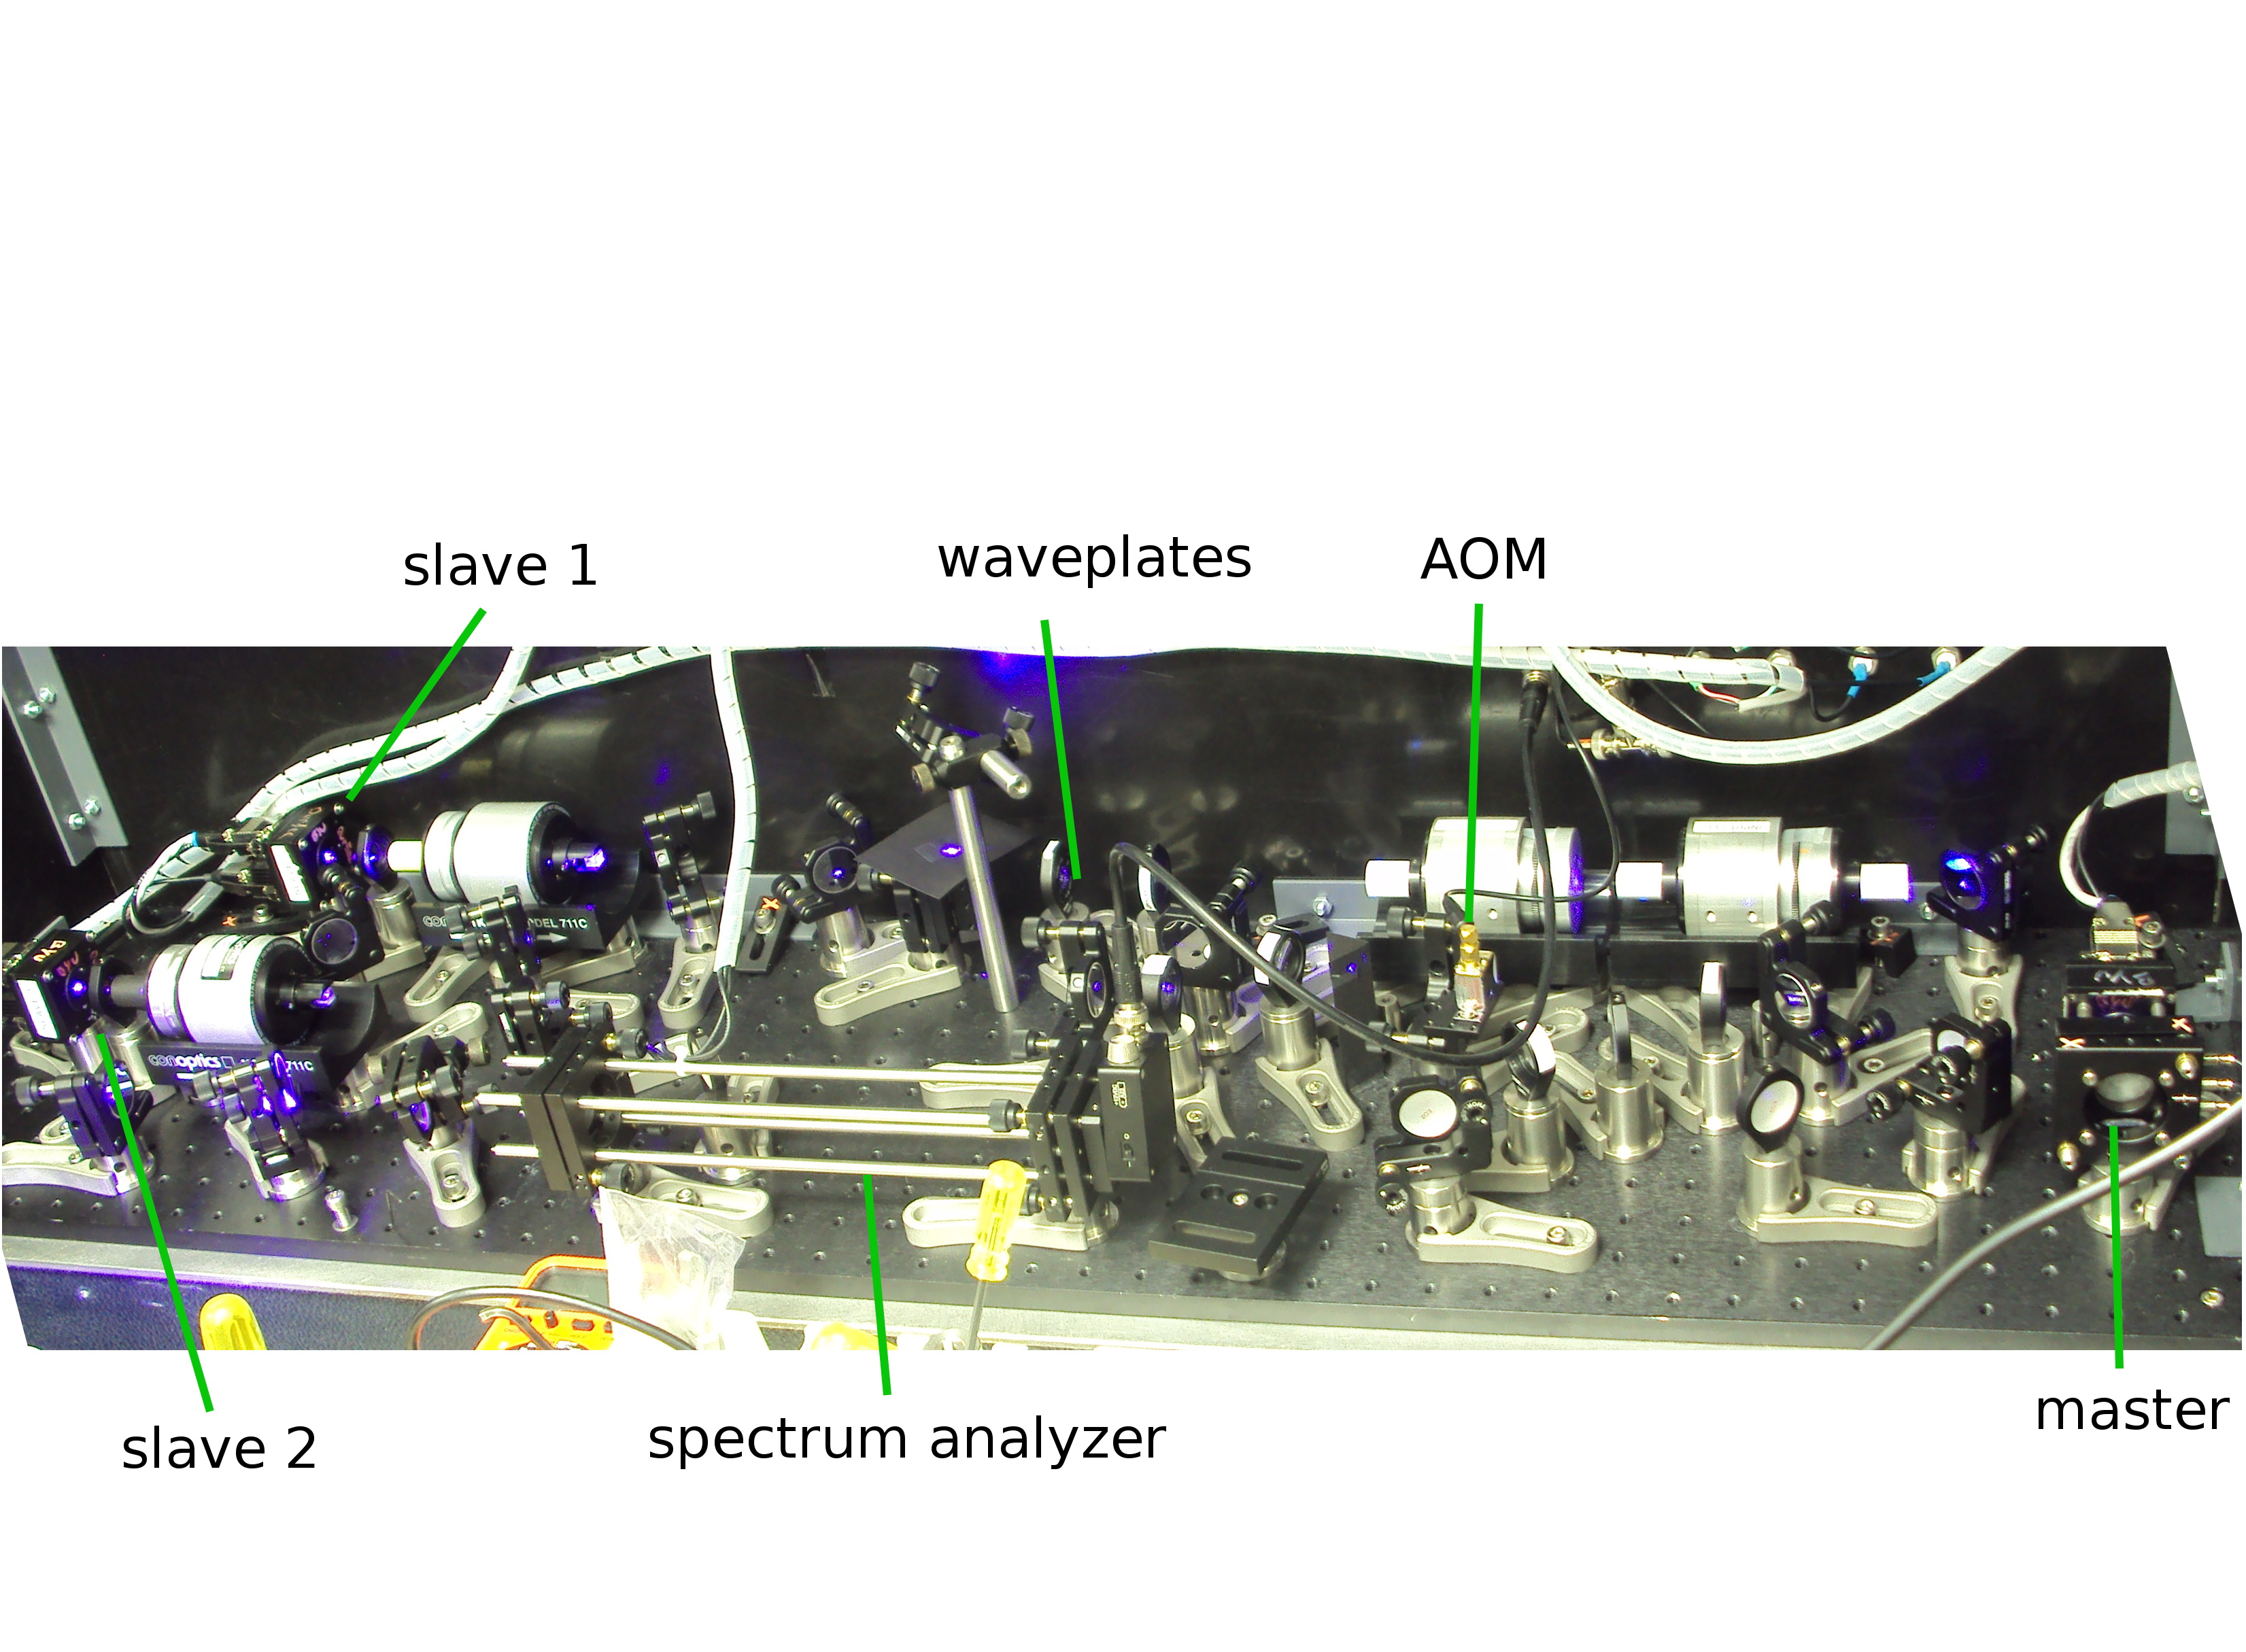
\includegraphics[width=1\textwidth]{entire_setup}}
    \caption[Photo of entire laser system]{\label{fullexperimentphoto}
A photograph of the entire laser system while in operation.
    }
\end{figure}

There are three separate laser diodes in housings. One of them is designated the ``master'' laser. The other two are designated ``slave 1'' and ``slave 2.'' The light that will actually be used on the atoms in the experiment is generated by the two slave lasers (slave 1 and slave 2).
 A diagram of the main components of the system can be found in Figure\,\ref{diagramOfSetup3} while a picture of the completed setup can be found in Figure\,\ref{fullexperimentphoto}. 

The system is designed so that some small fraction of the light coming from the master laser is shifted in frequency by an Acousto Optic Modulator (AOM) and used to seed one of the slave lasers. The unshifted light passing through the AOM is then retroreflected so that it passes through the AOM in the opposite direction and some small fraction of this light is then shifted in the opposite direction. This light is used to seed the other slave laser. Coupling the shifted light into the slave lasers and adjusting the slave lasers in such a way that they lase in a mode that is resonant with the light coupled into them is what is meant by ``injection locking.'' 

The advantage of this setup is that as the frequency of the master laser drifts, both slaves will drift with it, while the relative frequency difference between the slave lasers will remain stable.  As I will later show in Chapter \ref{ChapterAboutTheAtoms}, the experiment is less sensitive to common mode drift between the two slave lasers than it is to drifts of the individual slaves relative to one another. 

%However, the difference in frequency between the slave lasers is set by an RF function generator with sub-Hz precision.

 %The master laser serves as a stable frequency reference so that the slave lasers can be seeded by it. 
Thus, the basic objectives that I accomplished were (1) to make a stable master laser tuned near the mean of the frequencies that we desire out of the slave lasers, (2) to shift the light from the master laser using an AOM (3) to injection lock the slave lasers, and (4) to calculate the powers and frequency offsets necessary for our experiment.

\begin{figure}
    \centerline{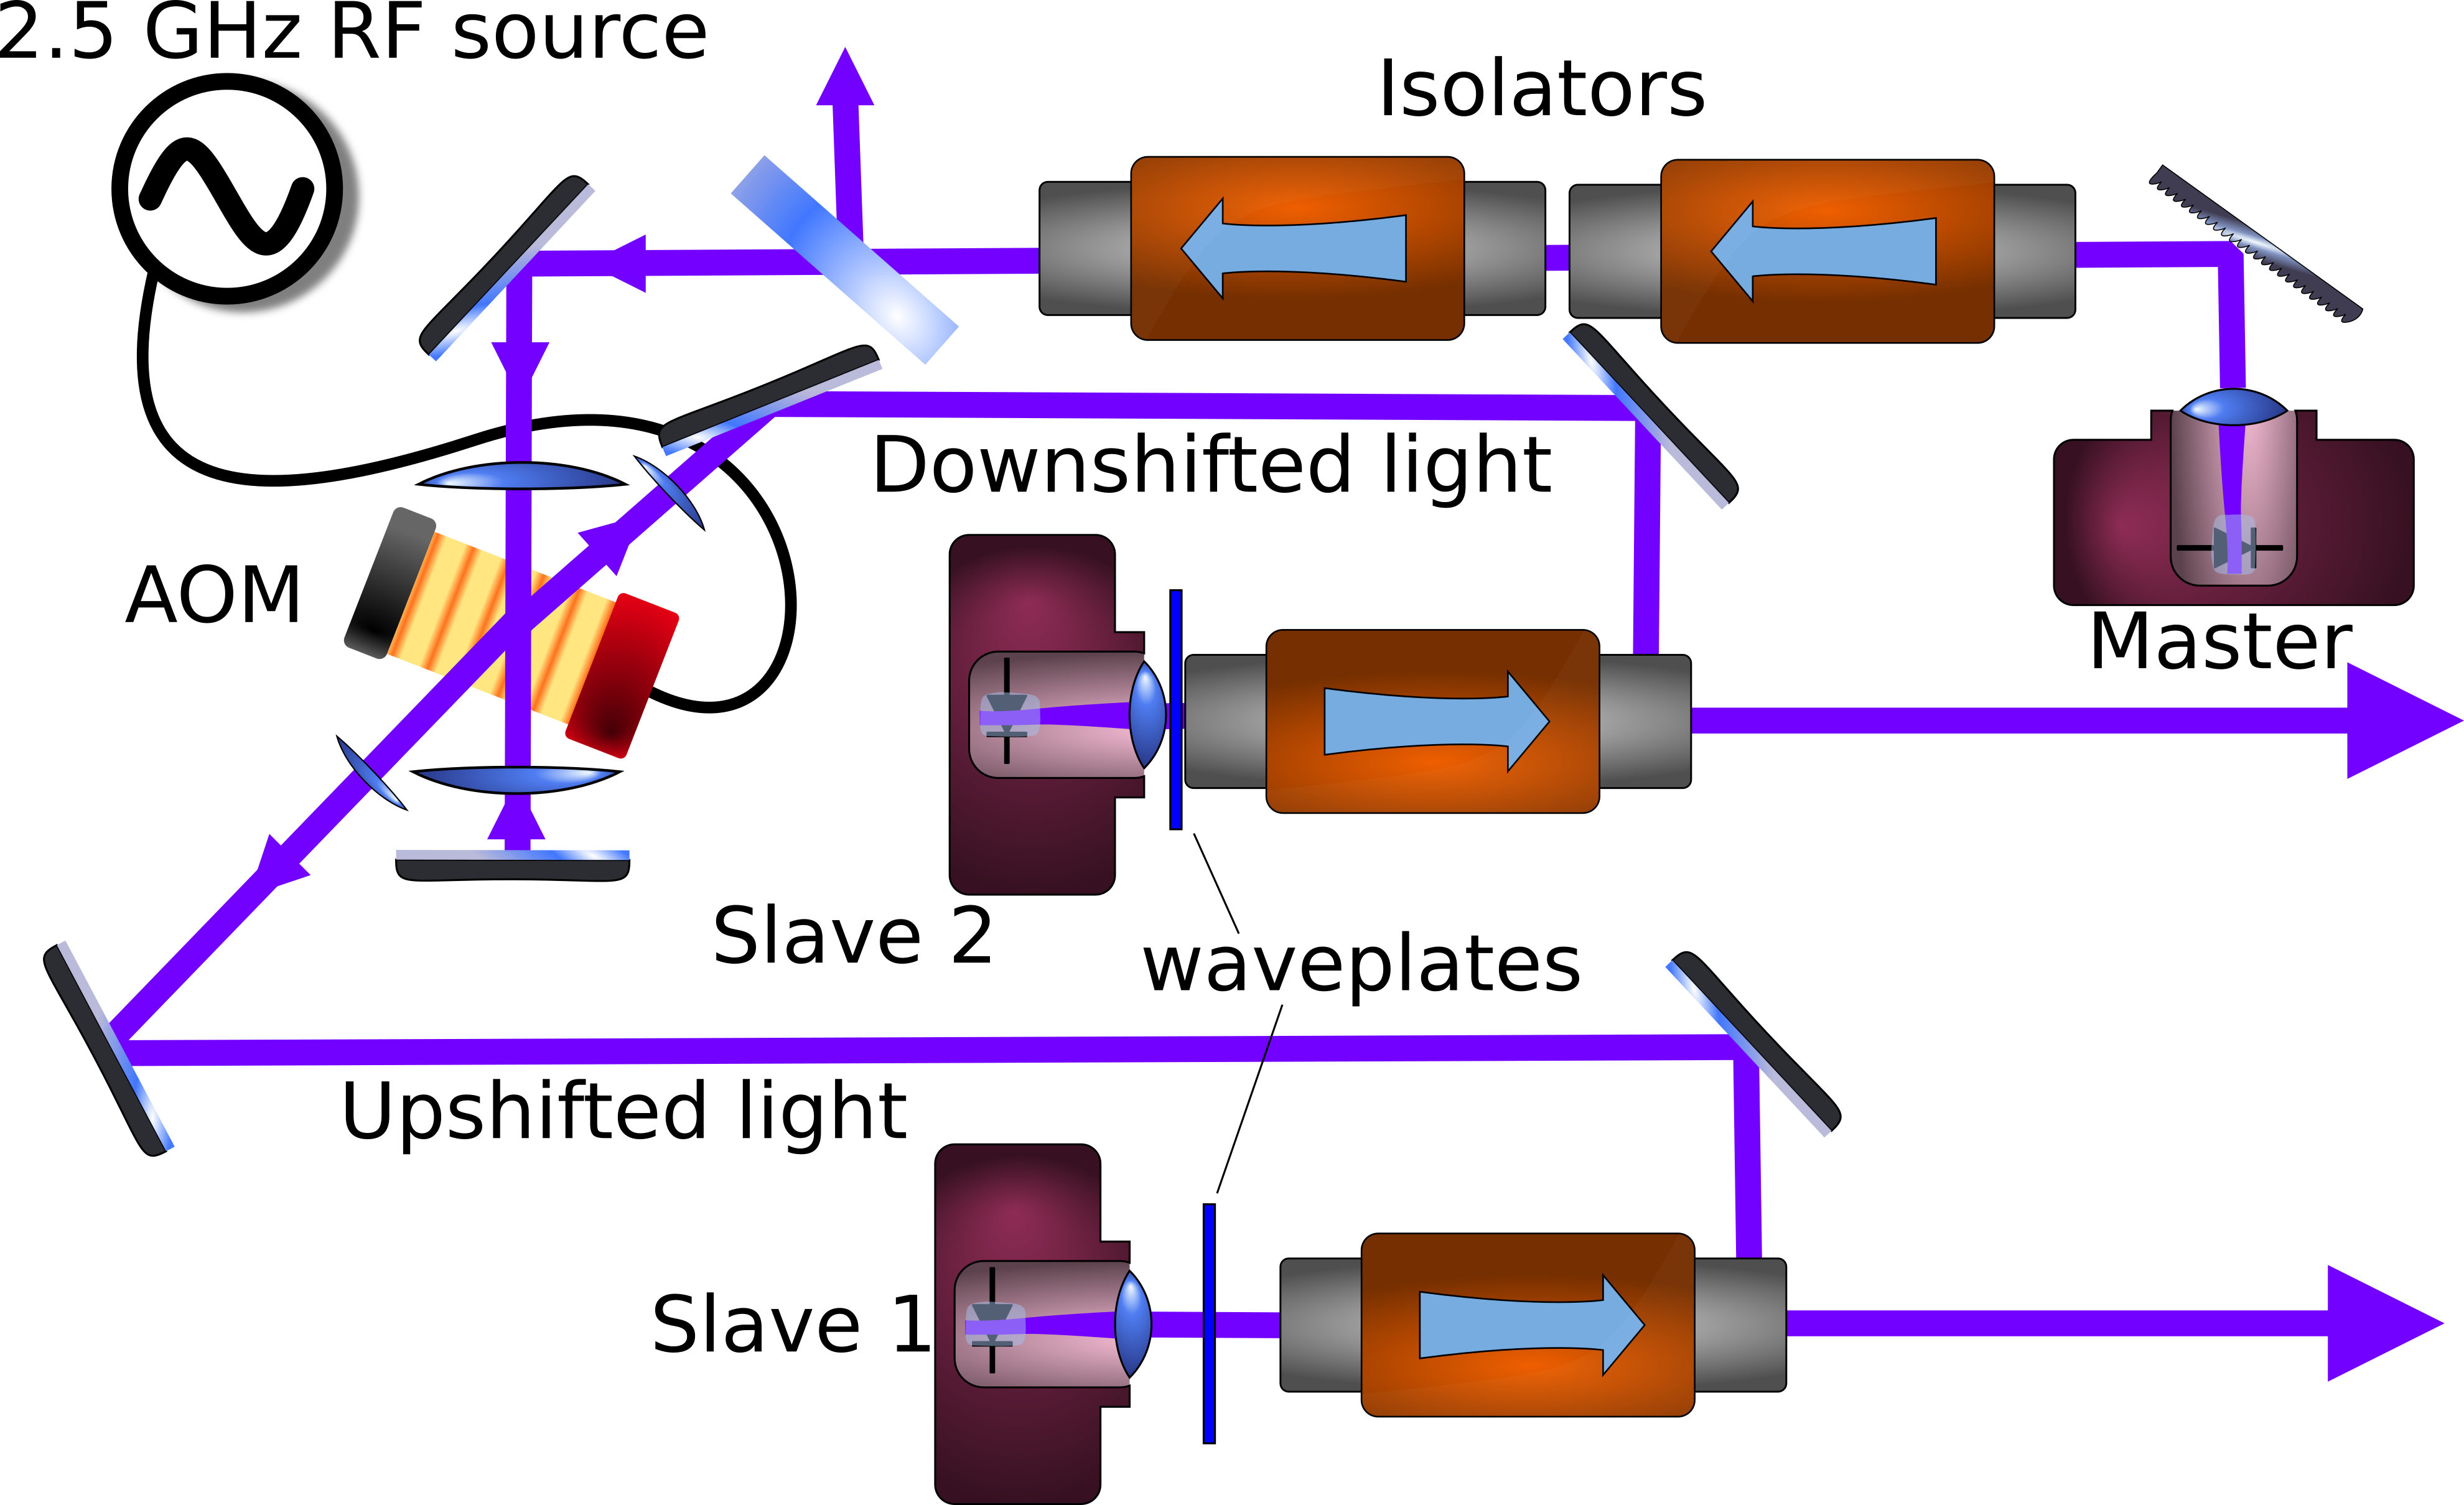
\includegraphics[width=1\textwidth]{diagramOfSetup3}}
    \caption[Schematic diagram of the laser system]{\label{diagramOfSetup3}
	A schematic diagram of the basic pieces of the 408 nm 5 GHz detuned laser system apparatus. The master laser is depicted on the upper right. Its beam passes through two optical isolators in series. After this, the AOM is depicted with the upshifted and downshifted light coming out at exaggerated angles. These beams are then coupled into the rejection ports of two other optical isolators. Half waveplates are mounted in front of each of the slave lasers to rotate the polarization of the light to match the input polarizers on the isolators. The beams that will be used in the experiment are shown exiting through the lower right side of the diagram. The waveplates and polarizing beam cube that are used to adjust the light coupling into the AOM are not depicted.
    }
\end{figure}
\section{Following the beam path}
Light from the master laser passes through two optical isolators. These use Faraday rotation and a pair of glan polarizers to ensure that light travelling away from the master laser is allowed to propagate while light is prevented from coming back into the master laser. See Fig.~\ref{isolatorPicture}.

\begin{figure}
\centerline{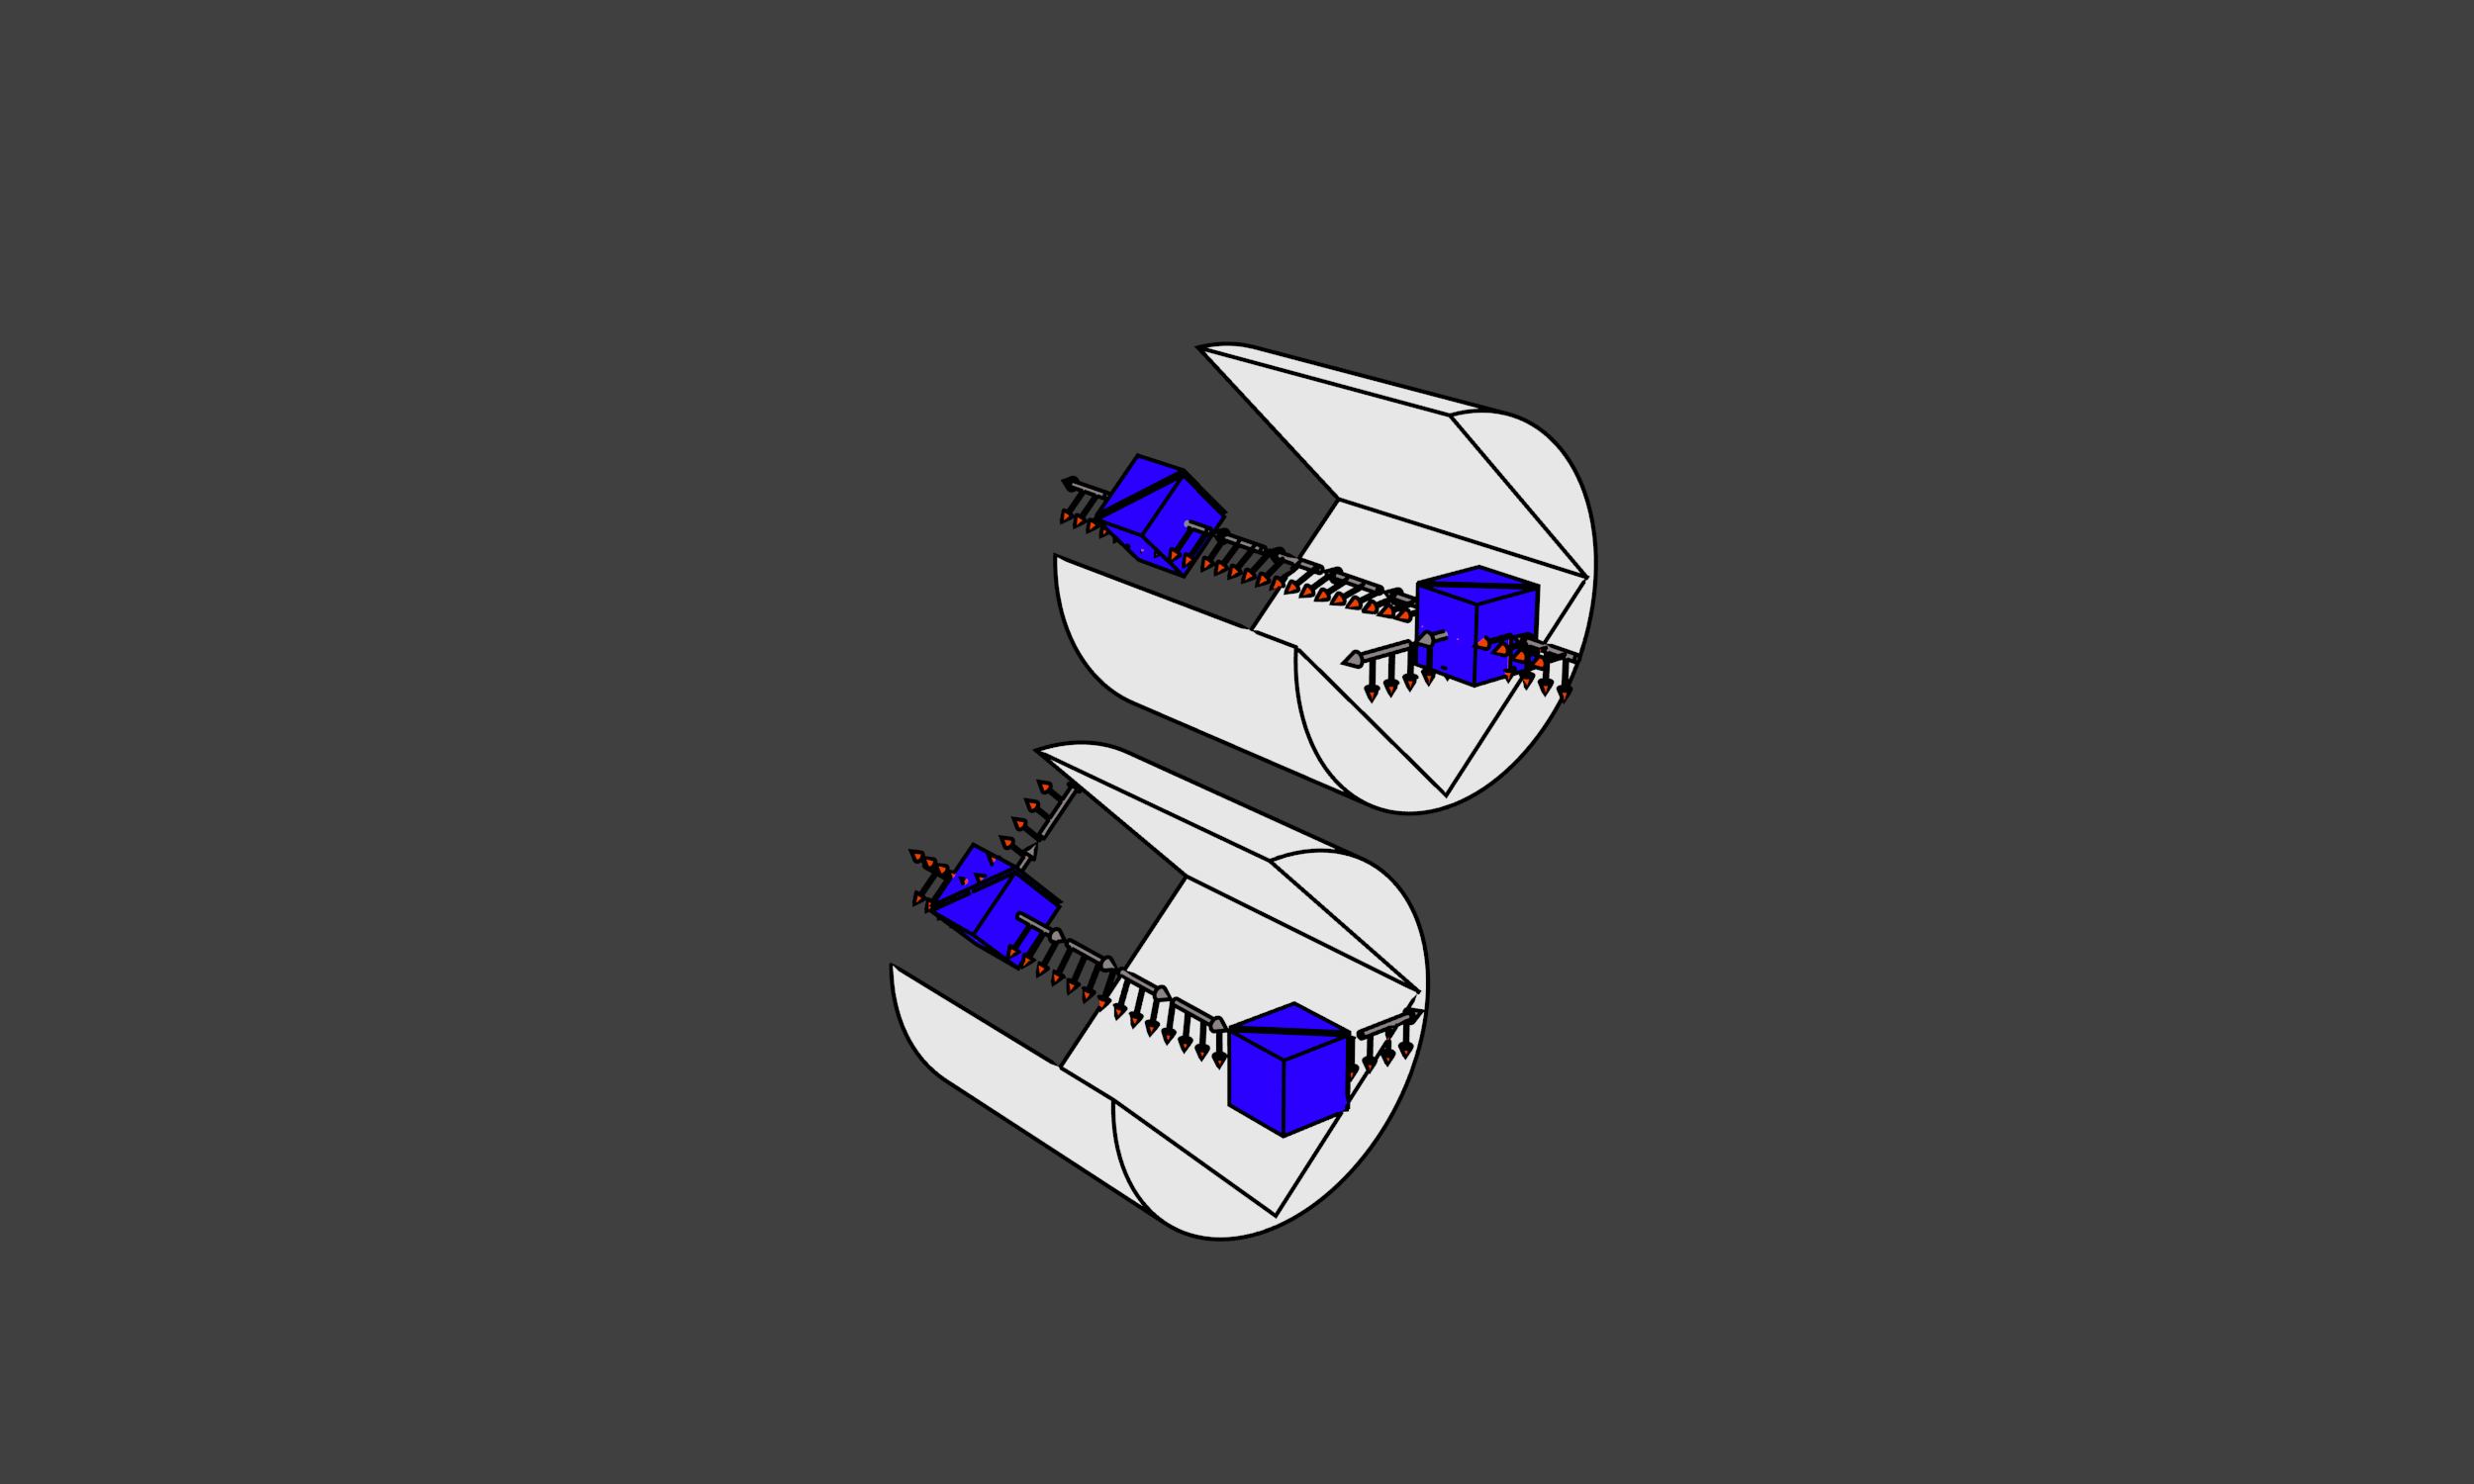
\includegraphics[width=1\textwidth]{isolators}}
\caption[Optical isolator illustration]{\label{isolatorPicture} Optical isolators work via Faraday rotation of the light. The Faraday effect occurs in certain materials when placed under a strong magnetic field. The Faraday effect results in the rotation of the polarization of light as it passes through a crystal. The direction of the change in polarization is depicted in the diagram. The image on the left shows an isolator rejecting light, while the image on the right depicts the same isolator allowing light travelling in the opposite direction to pass through.}
\end{figure}

Optical isolators are important because the stability of the master laser and the injection locking of the slave lasers requires control of the light being coupled into the laser cavity. By installing isolators, I can prevent unwanted reflections from coupling back into the master laser. This is an especially serious issue for the master laser since later in the beam path, the beam is retroreflected in such a way that, absent the isolators, light would couple directly back into the master laser. 

The beam then passes through a pair of waveplates and a polarizing beam cube, which serves the dual purpose of allowing us to attenuate the portion of the beam that goes through the AOM and splitting off a beam that can be used in our spectrum analyzer. A discussion of the method I used for adjusting the quantity of light passing through these waveplates can be found in Appendix \ref{twoWaveplateTrick}.

After this, the laser is passed twice through an Acousto-optic Modulator (AOM). The first-order diffracted beam from the first pass through the AOM produces light that is shifted up in frequency (down in wavelength). However, most of the power is contained in the 0th order beam that passes through the AOM without being shifted at all. I collimate the 0th order beam and retroreflect it, thereby sending it through the AOM in the opposite direction. This pass produces a weak beam that is downshifted in frequency. I thus end up with two beams, one of which is shifted upwards by 2.5 GHz relative to the master laser and the other of which is shifted downward by 2.5 GHz. 

These two shifted beams are then coupled into the two slave lasers. The slave lasers amplify this light and lase in a mode that is resonant with the shifted light. Coupling the seed light to the slave laser cavities requires that the incoming seed light propagate along the same path as the outgoing light from the slave laser. In order to achieve this, each slave laser has an optical isolator in its beam path. The optical isolator is configured to allow light emanating from the slave laser to come out its normal output port. However, the seed light is coupled to the laser by shining it through one of the rejection ports of the isolator (i.e. one of the ports that light with the wrong polarization or light travelling the wrong direction is siphoned towards). In this way, we are able to create overlapping, counterpropagating beams with the correct polarizations (the polarization of the seed light pretty much matches the polarization of the light generated by the laser). The polarization considerations are not totally trivial, but the polarization of the light is crucial to understanding how the isolator works and why the isolator is necessary. However, whether the optical isolator is used for rejecting light that is propagating in the wrong direction, or whether it is used to couple light into a laser, in either case it is allowing light with the same polarization at one port to travel along different paths depending on the direction the light is propagating. 
These considerations are explained more deeply in Chapter\,\ref{InjectionLockingChapter}. 
%Is that true? Do I explain it very well? 

The outputs of these two lasers are what we will send to the ion interferometer experiment to stimulate Raman transitions. Some of the light from each of the slaves are also redirected to the spectrum analyzer using beamsplitters or, for the purposes of characterization, mirrors that will later be removed.

%We could have maybe used light coming out the rejection ports to monitor second order effects from the AOM. 

\begin{figure}
%    \centerline{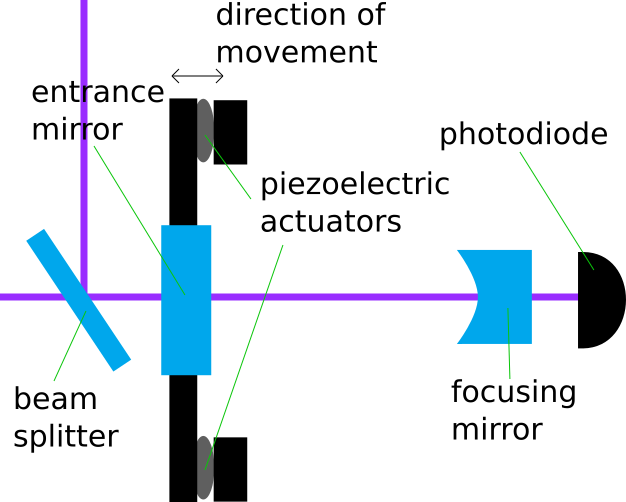
\includegraphics[trim=100pt 100pt 100pt 100pt, clip=true, totalheight=0.5\textheight,angle=90]{spectrumAnalyzer}}
    \centerline{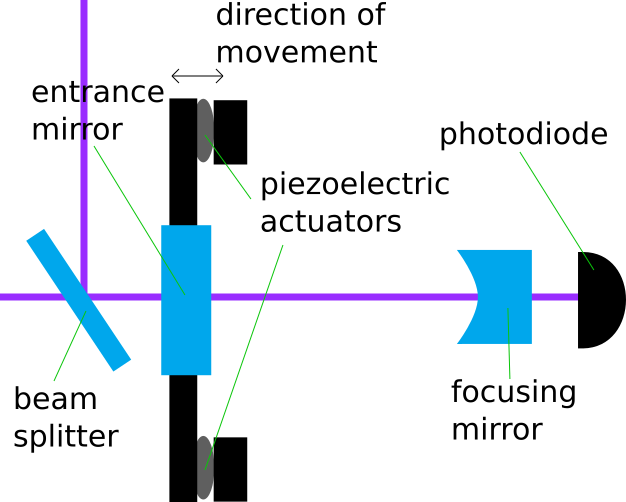
\includegraphics[totalheight=0.3\textheight ]{spectrumAnalyzer}}
    %\includegraphics[totalheight=0.3\textheight]{testfigure}
    \caption[Spectrum analyzer diagram]{\label{fig:spectrumAnalyzer}
    A diagram of the spectrum analyzer. The spectrum analyzer consists of a Fabry-Perot cavity of adjustable length. The photodiode on the far right of the diagram outputs a signal that shows when the incoming lasers are resonant. The left cavity mirror is mounted on a piezoelectric mount that allows us to finely displace the mirror using electronic controls. There is a beamsplitter before the cavity that allows us to couple two different lasers to the cavity at the same time. Elsewhere in the system, there is a removable mirror that can be used to select which lasers are coupled to the cavity. A mirror on a flip mount (not shown) allows either the master laser and one slave laser or either of the two slave lasers to be coupled to the cavity simultaneously.
}
\end{figure} 

\section{Verifying the output of the 408 nm 5GHz detuned laser system}
\label{spectAnalayzer}
I use a Fabry-Perot spectrum analyzer to monitor whether the slaves are injection locked and to verify that the master laser and slave lasers are running single mode. The spectrum analyzer is depicted in Fig.\,\ref{fig:spectrumAnalyzer}. 
The spectrum analyzer is a semiconfocal cavity of length 200 mm whose length can be varied electronically. The flat, partially reflective mirror through which light enters the cavity is mounted on a Thorlabs KC1-PZ Kinematic Mirror Mount that features piezo-electric actuators. This allows for fine control of the mirror's position (and therefore fine changes in the cavity length). At the other end of the cavity there is a curved mirror of focal length 200 mm. Behind this there is a photodiode \footnote{the Thorlabs DET family of reversed biased photodiode products}.

The piezoelectric actuators are connected to a commercially available piezo control box that sweeps the voltage in a sawtooth wave type pattern with a frequency $\sim$20Hz. I use this to modulate the length of the cavity. When the cavity length is such that the coupled light is close to a resonance of the cavity, more light transmits through the cavity and there is a higher signal on the photodiode. 

The cavity moves far enough that light at any given frequency will go in and out of resonance several times over any given sweep of the piezoelectric actuators. In order to understand the repeating pattern of peaks, one must understand the free spectral range (FSR) of the cavity. The free spectral range (FSR) of the cavity is defined as the spacing between adjacent resonant frequencies of the cavity. Therefore, if $f$ is some frequency of light that is resonant with a cavity, $f+m\times \textnormal{FSR}$ will also be a resonant frequency of the cavity for any integer $m$. In the case of a hemiconfocal cavity like the one used in our setup, the free spectral range is given by 

\begin{equation}
    \textnormal{FSR}=\frac{c}{8L}
\end{equation}.

If I have a single frequency of light coupling to the cavity, I expect to see the same peak repeated several times as the laser comes into and out of resonance. In the case of our cavity (a semiconfocal cavity of length $20cm$), the period over which this pattern repeats is approximately the free spectral range, which in this case is 187 MHz. Thus, I can use the spectrum analyzer to place upper limits on the linewidth of the lasers. 

Furthermore, the spectrum analyzer is good for monitoring relatively small shifts in the frequencies of the lasers that are coupled to it. If I shift the frequency of one of the lasers, the location of its corresponding peak within the scan should also shift. 
By exploiting this, I can verify that the slave lasers track with the master laser: if I couple a slave laser and the master laser to the spectrum analyzer simultaneously and then scan the frequency of the master laser, I should see that the peaks corresponding to both the master laser and the slave laser move together and stay a fixed distance apart. 
This fact can also be used to verify that the relative offset of the slaves depends in the correct way on the frequency of the signal used to drive the AOM. I can couple slave 1 and slave 2 to the spectrum analyzer and then change the frequency on the RF frequency generator that is used to drive the AOM. The result should be that the relative location of the peaks corresponding to slave 1 move relative to the peaks that correspond to slave 2. Data showing both of these phenomena can be found in Chapter \ref{triumphantDataChapter}. A more complete discussion of the spectrum analyzer can be found in Appendix \ref{spectrumAnalyzer}. 
